\section{Introdução}

O objetivo deste trabalho é de realizar processamentos básicos de imagem e se familiarizar com Python e suas ferramentas. Pensando nisso, o programa desenvolvido utiliza a biblioteca OpenCV para leitura, codificação e decodificação de imagens PNG e usa Numpy para tratamento vetorizado da imagem.

Todos os processamentos serão aplicados nas mesmas imagens da especificação do trabalho e uma imagem colorida, apresentada na \cref{fig:color}.

\begin{figure}[H]
    \centering
    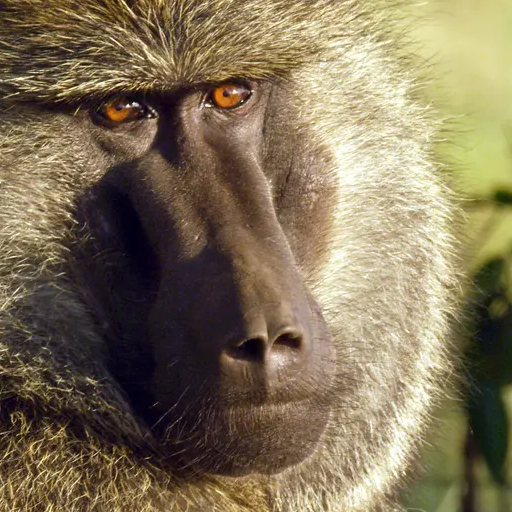
\includegraphics[width=6cm]{imagens/color.png}

    \caption{Imagem colorida usada como comparação dos resultados dos processamentos.}
    \label{fig:color}
\end{figure}

\section{O Programa}

\subsection{Código Fonte}

O programa foi desenvolvido em 4 arquivos separados:

\begin{description}
    \item[main.py] É o corpo do programa, resposável por processar os comandos e opções da linha de comando.

    \item[inout.py] Funções que tratam da entrada e saída do programa, como leitura e escritas de arquivos de imagem e também da apresentação da imagem em uma janela gráfica.

    \item[lib.py] Funções de tranformação da imagem, como ajute de brilho e acesso do plano de bits.

    \item[tipos.py] Definição dos tipos para tipagem estática (apenas o protocolo \autocite{ref:pep544} \pyline{Image}).
\end{description}

A tipagem estática é aplicada para facilitar o desenvolvimento e a leitura do código, mas ela limita a execução em Python para as versões 3.7 ou superior \autocite{ref:pep563}.

Todas as figuras base utilizadas neste relatório podem ser encontradas na pasta \texttt{imagens}. A \cref{fig:color}, por exemplo, está em \texttt{imagens/color.png}.

\subsection{Execução}

A execução deve ser feita através do interpretador de Python 3.7+. A única entrada obrigatória é o caminho para a imagem PNG que será processada. As entradas seguintes serão tratadas como comandos de processamento da imagem. Ao final da execução, a imagem resultante será exibida na tela. Por exemplo, o comando abaixo exibe na tela a \cref{fig:execucao}.

\begin{minted}{bash}
    $ python3.8 main.py imagens/color.png monocromatico plano.bit 6 negativo \
        mosaico padrao.txt
\end{minted}

\begin{figure}[H]
    \centering
    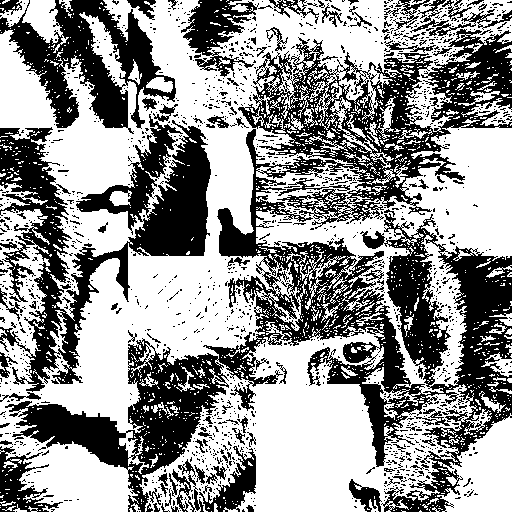
\includegraphics[width=6cm]{resultados/execucao.png}

    \caption{Aplicação de alguns processamentos na \cref{fig:color}.}
    \label{fig:execucao}
\end{figure}

Além das entradas posicionais, existem dois argumentos opicionais. Com \mintinline{bash}{--output}, ou \mintinline{bash}{-o}, é possível gravar o resultado em um arquivo PNG em vez de exibir na tela. O comando abaixo resulta na mesma imagem da \cref{fig:execucao}, mas guarda em um arquivo \texttt{out.png}, sem exibir na tela.

\begin{minted}{bash}
    $ python3.8 main.py imagens/color.png -o out.png monocromatico plano.bit 6 \
        negativo mosaico padrao.txt
\end{minted}

Se é desejável tanto a exibição da imagem quanto o salvamento no arquivo, o argumento \mintinline{bash}{--force-show} ou \mintinline{bash}{-f} pode ser usado.

\subsection{Comandos Entendidos}

O programa entende dez comandos distintos, apresentados abaixo, que podem ser repetidos quantas vezes forem necessárias. Os comandos são executados na ordem em que aparecem na linha de comando.

Todos os comandos abaixos devem ser usados da mesma forma como aparecem aqui, em letras minúsculas, sem acentos e com ponto onde aparecer abaixo. Os nomes em letras maiúsculas são os argumentos daquele comando, que devem aparecem após o nome do comando (a maioria deles não tem argumentos).

\begin{description}
    \item[\texttt{monocromatico}] Transforma a imagem para monocromática, em escala de cinza. Só faz diferente para entradas coloridas.

    \item[\texttt{negativo}] Inverte a intensidade de cada pixel da imagem, em todos os canais de cores.

    \item[\texttt{esp.verical}] Faz o espelhamento vertical da imagem.

    \item[\texttt{conv.intervalo}] Converte o intervalo de intensidades para [100, 200].

    \item[\texttt{inverte.pares}] Inverte a direção dos píxeis das linhas pares da imagem.

    \item[\texttt{reflexao}] Faz a reflexão das linhas superiores.

    \item[\texttt{aj.brilho GAMA}] Aplica um ajuste de brilho com fator \texttt{GAMA}.

    \item[\texttt{plano.bit M}] Extrai o plano de bit de ordem \texttt{M} para ordens em [0, 8).

    \item[\texttt{combina IMAGEM ALPHA}] Faz a combinação com outra imagem PNG no arquivo \texttt{IMAGEM} por média ponderada com um fator de peso \texttt{ALPHA}.

    \item[\texttt{mosaico ORDENACAO}] Contrói um mosaico da imagem a partir de nova ordem dos blocos descrita no arquivo \texttt{ORDENACAO} (detalhes na \cref{sec:mosaico}).
\end{description}
